\documentclass[10pt,a4paper]{article}
\usepackage[utf8]{inputenc}
\usepackage{amsmath}
\usepackage{amsfonts}
\usepackage{amssymb}
\usepackage{graphicx}

\title{Reporte 6}
\author{Antonio Cota Rodr\'iguez}
\date{}

\begin{document}

\maketitle{}

\section*{Introducci\'on}
En \'este reporte estudiaremos los efectos que tiene la resitencia del aire para movimientos par\'abolicos donde tambi\'en act\'ua la fuerza de gravedad y se desprecian alguna otra fuerza externa que afecte en nuestro an\'alisis. Se calcular\'a la diferencia entre el alcance m\'aximo de un tiro par\'abolico con resistencia y el otro sin \'esta. Se brindar\'a apoyo gr\'afico para ilustrar mejor la diferencia entre los tiros.

\section*{Teor\'ia}

Usualmente se asume que los efectos de la resistencia del aire son despreciables. Cuando se omite la resistencia del aire, la \'unica fuerza actuando sobre un proyectil de masa $m$   es igual a su peso, por lo que la componente de la aceleraci\'on en el eje $X$ es cero.

Sin embargo, la resistencia del aire (fuerza de arrastre) tiene un mayor efecto sobre el movimiento de diversos objetos.  Cuado \'esta se incluye en el c\'alculo, la fuerza de arrastre es aproximadamente proporcional al cuadrado de la rapid\'ez relativa del proyectil respecto al aire:
$$f=Dv^2,$$
donde $D$ es una constante que depende de la densidad del aire $\rho$, el coeficiente de arrastre del proyectil $C$ y su secci\'on transversal $A$ del objeto
$$D=\frac{\rho C A}{2}.$$
Para bolas esfericas el valor del coeficiente de arrastre es $C \approx 0.47$. Ahora, considerando la fuerza causada por la resistencia del aire y la gravedad, los componentes de la aceleraci\'on del proyectil son:
$$a_x=-(D/m)vv_x, \qquad a_y=-g-(D/m)vv_y,$$.
Debido a esto, la velocidad en $x$ tampoco es constante. Las componentes de la velocidad a cada instante de tiempo son
$$v_x + \Delta v_x = v_x + a_x \Delta t, \qquad 
v_y + \Delta v_y = v_y + a_y \Delta t,$$

y finalmente, las coordenadas en cada instante de tiempo se calculan con las ecuaciones
$$x + \Delta x = x + v_x \Delta t + \frac{1}{2} a_x (\Delta t)^2, \quad y + \Delta y = y + v_y \Delta t + \frac{1}{2} a_y (\Delta t)^2.$$

\section*{C\'odigo en Fortran}

A continuaci\'on se mostrar\'a el c\'odigo que se utiliz\'o en Fortran y un screenshot de \'este en ejecuci\'on.   

\begin{verbatim}

Subroutine POSICION(x1,y1,vx,vy,axi,ayi,dti,x2,y2)
Implicit None
real :: x1,y1,vx,vy,axi,ayi,dti,x2,y2

x2= x1 + vx*dti + 0.5*axi*dti*dti

y2= y1 + vy*dti + 0.5*ayi*dti*dti

End Subroutine POSICION

!------------------------------------------------------

Subroutine ARRASTRE(g,Di,mi,vx,vy,axi,ayi)
Implicit None
real :: g,Di,mi,vx,vy,axi,ayi

 axi = -(Di/mi) * vx * vx
 ayi = -g - (Di/mi)*vy*vy

End Subroutine ARRASTRE

!------------------------------------------------------

program projectile_drag  
       implicit none  

! DECLARACION DE VARIABLES
       real :: u, a, t_max, a_grados, D, rho, C, At
       real :: x0, y0, vx0, vy0,  ax, ay, m,r
       real :: xi,xii,yi,yii,yi2
       real :: x(1000),y(1000)  
          integer :: i = 0
          real :: t=0, dt=0.05


! DECLARACION DE CONSTANTES
       real, parameter :: pi = 4.0*atan(1.0) 
       real, parameter :: g = 9.81

       write(*,*) 'Densidad del fluido: '
       read *, rho
       write(*,*) 'Radio de la esfera: '
       read *, r
       write(*,*) 'Masa:'   
       read *, m

       C=0.47
       At= pi*r*r
       D = rho*C*At/2.0
     

       write(*,*) 'Angulo inicial:'   
       read *, a_grados   
       write(*,*) 'Velocidad inicial:'   
       read *, u   
       write(*,*) 'Posicion inicial x:'   
       read *, x0   
       write(*,*) 'Posicion inicial y:'   
       read *, y0
 

!CONVERTIR ANGULO A RADIANES 
       a = a_grados*pi/180.0   
       
!COMPONENTES DE VELOCIDAD
       vx0 = u*cos(a)
       vy0 = u*sin(a)

!!!!
       t_max= 2000*dt
       xi=x0
       yi=y0

!ABRIR ARCHIVO .DAT
       open(1, file='drag.dat')   
 
!CALCULO DE LA TRAYECTORIA CON RESISTENCIA DEL AIRE        
       do              
            call  ARRASTRE(g,D,m,vx0,vy0,ax,ay)
            call  POSICION(xi,yi,vx0,vy0,ax,ay,dt,xii,yii)
             if (yi<0) then
               exit
            end if
!ESCRIBIR CON FORMATO
            write(1,1000) xi, yi
            1000 format (2f8.2)
!REDEFINIR VARIABLES
            vx0 = vx0 + ax*dt
            vy0 = vy0 + ay*dt
            xi=xii
            yi=yii
       end do   
       close(1)


!CALCULO DE LA TRAYECTORIA SIN RESISTENCIA DEL AIRE
!(SE CONSIDERA D=0 Y SE TOMAN VALORES INICIALES x(0), y(0), u)
       
       vx0 = u*cos(a)
       vy0 = u*sin(a)
       xi=x0
       yi2=y0
       dt=0.1

       open(1, file='nodrag.dat')   
 
       do              
            call  ARRASTRE(g,0.0,m,vx0,vy0,ax,ay)
            call  POSICION(xi,yi2,vx0,vy0,ax,ay,dt,xii,yii)

             if (yi2 < 0 ) then
               exit
            end if
!ESCRIBIR CON FORMATO
            write(1,1001) xi, yi2
		1001 format (2f8.2)
!REDEFINIR VARIABLES
            vx0 = vx0 + ax*dt
            vy0 = vy0 + ay*dt
            xi=xii
            yi2=yii
       end do   
       
       close(1)

       

  
end program projectile_drag 

\end{verbatim}

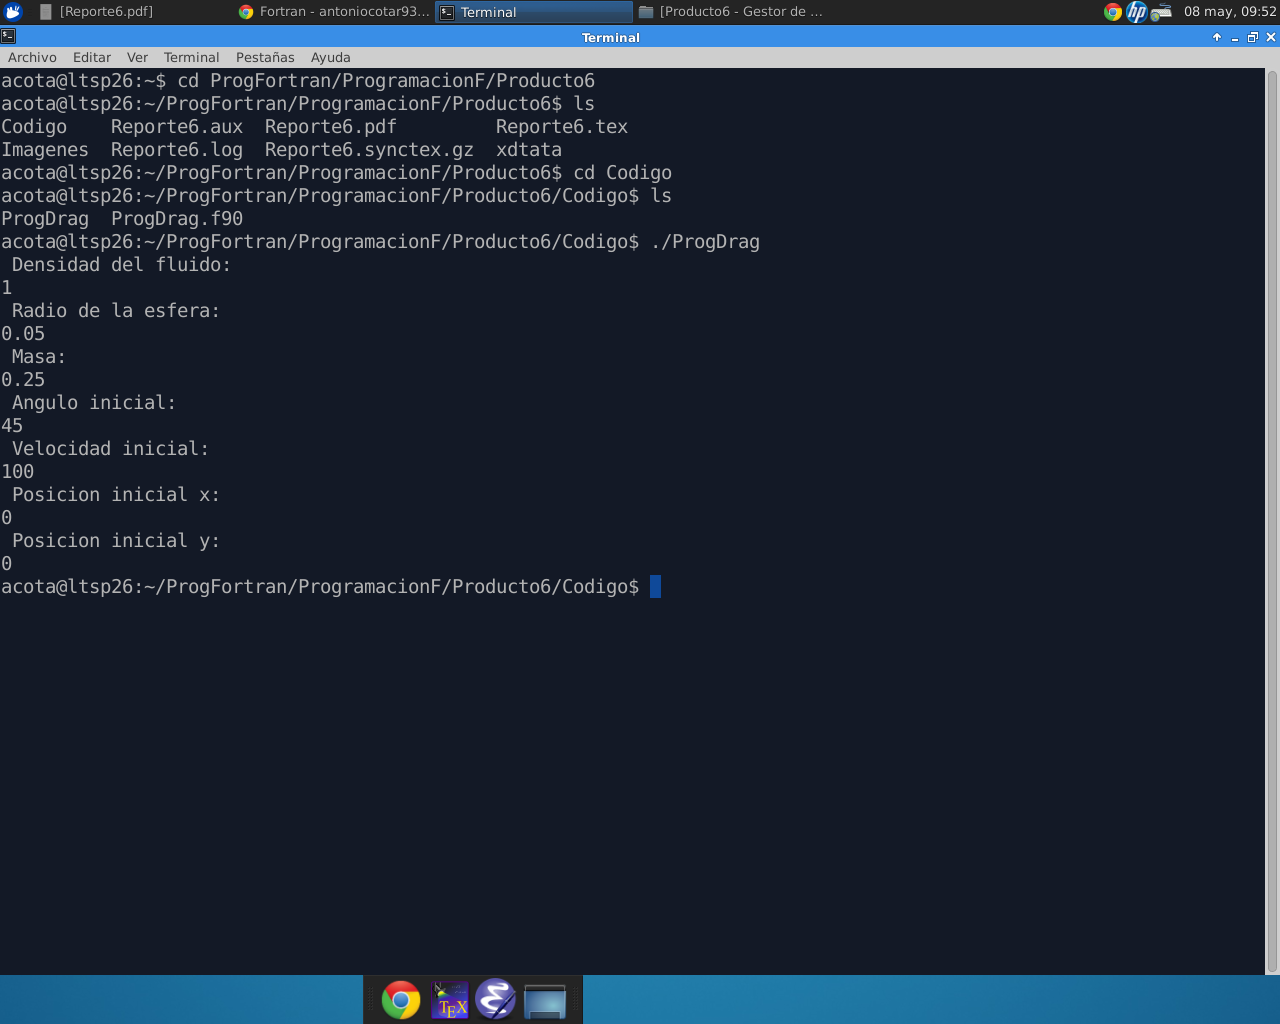
\includegraphics[scale=0.3]{Arrastre}


\section*{Gr\'aficas}

En esta secci\'on utlizamos el programa ''gnuplot'' para graficar los datos obtenidos por el programa que ejecutamos para diversos \'angulos (30,45,60 grados)

\begin{itemize}
\item 30 grados
\\\\
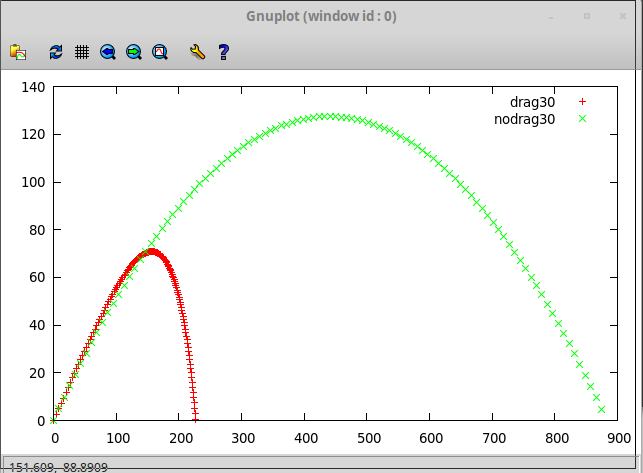
\includegraphics[scale=0.5]{30grados}

\item 45 grados
\\\\\\
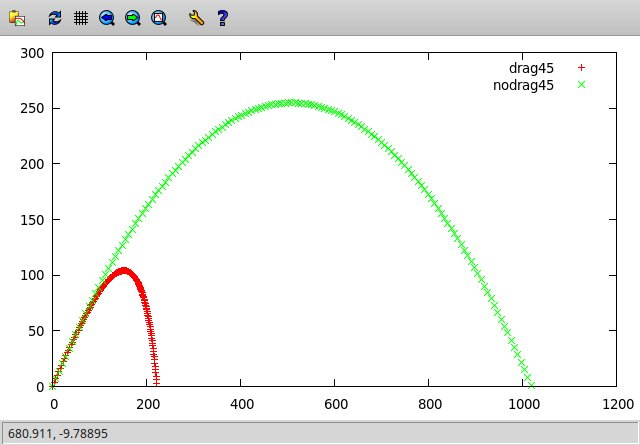
\includegraphics[scale=0.5]{45grados}

\item 60 grados
\\\\
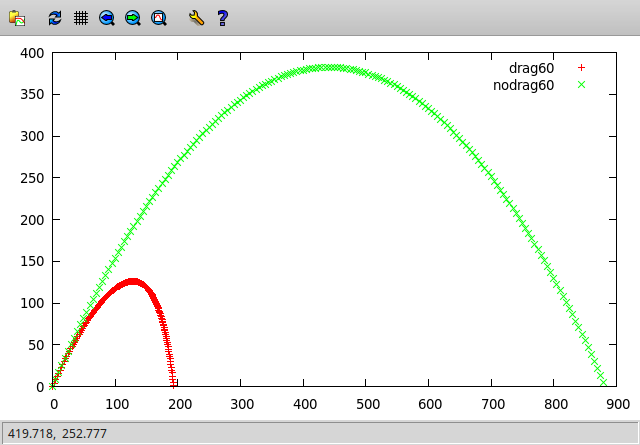
\includegraphics[scale=0.5]{60grados}

\end{itemize}

\section*{Diferencia y Error Porcentual}

\begin{itemize}
\item \'Angulo de 30 grados
\\\\
Alcance m\'aximo con arrastre = 227.31\\
Alcance m\'aximo sin arrastre = 874.79\\
Diferencia = 647.48\\
error porcentual = 385\%\\

\item \'Angulo de 45 grados
\\\\
Alcance m\'aximo con arrastre = 221.63\\
Alcance m\'aximo sin arrastre = 1118.23\\
Diferencia = 896.6\\
error porcentual = 505\%\\

\item \'Angulo de 60 grados
\\\\
Alcance m\'aximo con arrastre = 193.10 \\
Alcance m\'aximo sin arrastre = 880.00\\
Diferencia = 686.9\\
error porcentual = 455\%\\



\end{itemize}






\end{document}